\documentclass[handout]{beamer}
%\documentclass[compress]{beamer}

% =========================
% Packages
% =========================
\usepackage[T1]{fontenc}
\usepackage[american]{babel}
\usepackage{csquotes}
\usepackage[style=apa, backend=biber]{biblatex}

\usepackage{pifont}
\usepackage{threeparttable}
\usepackage{subcaption}
\usepackage{tikz-qtree}
\usepackage{tikz}
\usepackage{multicol}
\usepackage{booktabs}
\usepackage{graphicx}
\usepackage{neuralnetwork}
\usepackage{hyperref}
\usepackage{fancyvrb}
\usepackage{xcolor}
\usepackage{minted}

% =========================
% Bibliography and graphics
% =========================
\addbibresource{../resources/literature.bib}
\graphicspath{{../resources/pictures/}}

% =========================
% Hyperref
% =========================
\hypersetup{
  pdfborder={0 0 0},
  colorlinks=true,
  pdfauthor={Anne Kroon, Saurabh Khanna},
  pdftitle={Computational Communication Science 2}
}

% =========================
% Theme
% =========================
\usetheme[block=fill,subsectionpage=progressbar,sectionpage=progressbar]{metropolis}

\definecolor{Purple}{HTML}{911146}
\definecolor{Orange}{HTML}{CF4A30}

\setbeamercolor{alerted text}{fg=Orange}
\setbeamercolor{frametitle}{bg=Purple,fg=white}
\setbeamercolor{structure}{fg=Purple}
\setbeamercolor{normal text}{bg=white,fg=black}

\setbeamercovered{still covered={\opaqueness<1->{5}},again covered={\opaqueness<1->{100}}}

\setbeamersize{text margin left=12pt,text margin right=12pt}
\setbeamertemplate{section page}[progressbar]
\setbeamertemplate{subsection page}[progressbar]
\setbeamertemplate{itemize item}{\color{Purple}$\bullet$}

\setbeamerfont{frametitle}{size=\Large,series=\bfseries}
\setbeamerfont{framesubtitle}{size=\normalsize}
\setbeamerfont{normal text}{size=\small}
\setbeamerfont{itemize/enumerate body}{size=\small}
\setbeamerfont{itemize/enumerate subbody}{size=\small}
\setbeamerfont{block title}{size=\large,series=\bfseries}

\renewcommand*{\bibfont}{\tiny}

% headline with navigation
\makeatletter
\setbeamertemplate{headline}{%
    \begin{beamercolorbox}[colsep=1.5pt]{upper separation line head}
    \end{beamercolorbox}
    \begin{beamercolorbox}{section in head/foot}
        \vskip2pt\insertnavigation{\paperwidth}\vskip2pt
    \end{beamercolorbox}%
    \begin{beamercolorbox}[colsep=1.5pt]{lower separation line head}
    \end{beamercolorbox}
}
\makeatother

% =========================
% Minted
% =========================
\usemintedstyle{colorful}
\setminted{
  breaklines,
  fontsize=\tiny,
  bgcolor=gray!5
}

% =========================
% Custom commands
% =========================
\newcommand{\question}[1]{
    \begin{frame}[plain]
        \begin{columns}
            \column{.4\textwidth}
            \makebox[\columnwidth]{%
                
\includegraphics[width=\columnwidth,height=\paperheight,keepaspectratio]{mannetje.png}}
            \column{.6\textwidth}
            \large
            \textcolor{Orange}{\textbf{\emph{#1}}}
        \end{columns}
    \end{frame}
}

\newcommand{\instruction}[1]{\emph{\textcolor{gray}{[#1]}}}

% =========================
% Presentation metadata
% =========================
\title{Computational Communication Science 2}
\subtitle{Week 1 -- Introduction \& Working with Textual Data}
\author{Anne Kroon \and Saurabh Khanna}
\institute{Digital Society Minor \\ University of Amsterdam}
\date{March 30, 2026}
\titlegraphic{
    \hfill
    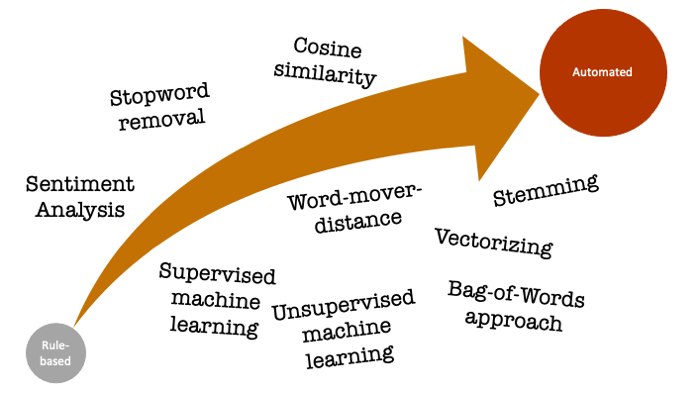
\includegraphics[width=0.32\linewidth]{Roadmap_terms.png}
}

\begin{document}

\begin{frame}
	\titlepage
\end{frame}

\begin{frame}{Today}
\begin{itemize}
	\item Course introduction
	\item What is Computational Communication Science?
	\item Why study text as data?
	\item Two ways to analyze text
	\item First steps in preprocessing
\end{itemize}
\end{frame}

\section[The people]{Introducing the teaching team}

\begin{frame}{Introducing\ldots \huge{Saurabh}} 
	\begin{columns}
		\column{.3\textwidth}
		\makebox[\columnwidth]{%
			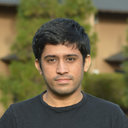
\includegraphics[width=\columnwidth,height=\paperheight,keepaspectratio]{Saurabh-Khanna-2.png}}
		\column{.7\textwidth}
		\textbf{dr. Saurabh Khanna} \\[0.2cm]
		Assistant Professor, Youth \& Media Entertainment
		\vspace{0.3cm}
		\begin{itemize}
			\item Studies how people understand information in a digital world
			\item Uses computational methods to study communication and media
		\end{itemize}
		\vspace{0.3cm}
		\textbar\ s.khanna@uva.nl \textbar\ \url{https://www.uva.nl/en/profile/k/h/s.khanna/s.khanna.html}
	\end{columns}
\end{frame}

\begin{frame}{Introducing\ldots \huge{Anne}} 
	\begin{columns}
		\column{.3\textwidth}
		\makebox[\columnwidth]{%
			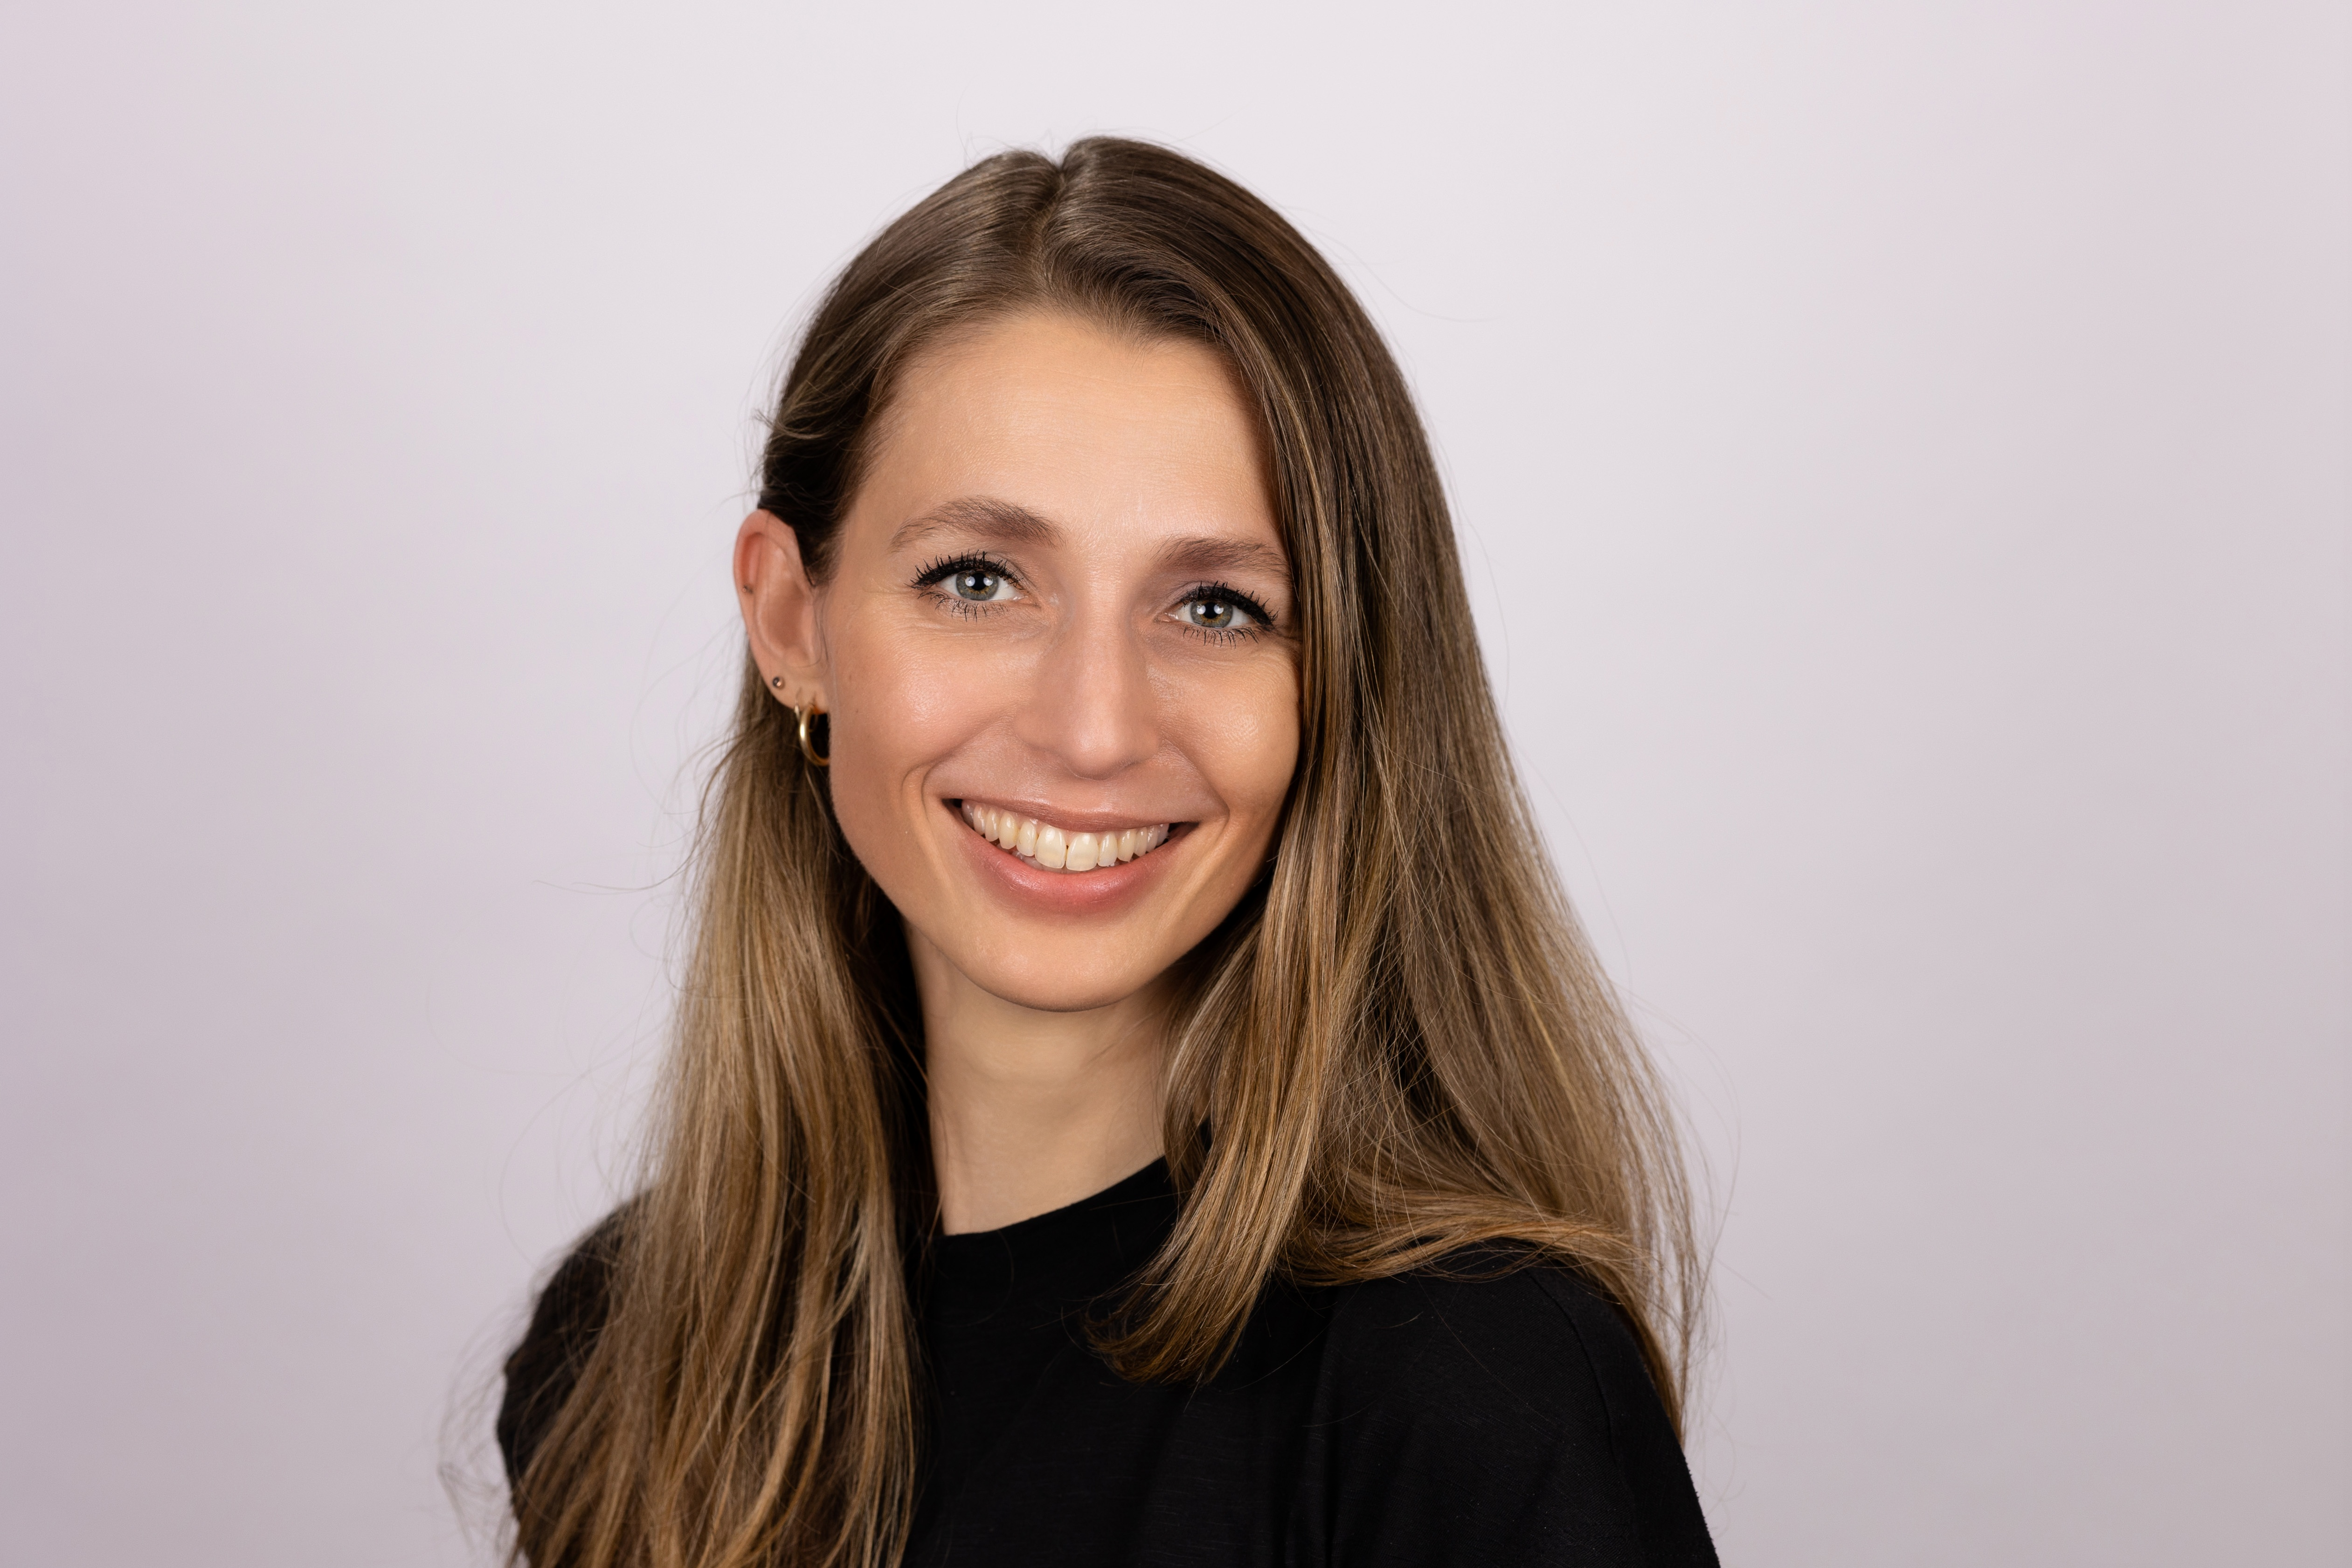
\includegraphics[width=\columnwidth,height=\paperheight,keepaspectratio]{anne.jpg}}
		\column{.7\textwidth}
		\textbf{dr. Anne Kroon} \\[0.2cm]
		Associate Professor, Communication, Organizations \& Society
		\vspace{0.3cm}
		\begin{itemize} 
			\item Research on biased AI in recruitment
			\item Research on media bias regarding minorities
			\item Works with text analysis and word embeddings
		\end{itemize}
		\vspace{0.3cm}
		@annekroon \textbar\ a.c.kroon@uva.nl \textbar\ \url{http://www.uva.nl/profiel/k/r/a.c.kroon/a.c.kroon.html}
	\end{columns} 
\end{frame}

\begin{frame}{Introducing\ldots \huge{Roeland}}
\begin{columns}
	\column{.3\textwidth}
	\centering
	\vspace{0.5cm}
	\Large Tutorials

	\column{.7\textwidth}
	\begin{columns}
		\column{.4\textwidth}
		\includegraphics[width=\linewidth]{roeland}

		\column{.6\textwidth}
		\textbf{Roeland Dub\`el} \\[0.2cm]
		Teaching the tutorial sessions
		\vspace{0.3cm}
		\begin{itemize}
			\item Helps with coding exercises and questions
			\item Supports your progress on the group assignment
			\item Best person to ask during tutorials when code does not work
		\end{itemize}
		\vspace{0.3cm}
		\textbar\ r.dubel@uva.nl
	\end{columns}
\end{columns}
\end{frame}

\section[The course]{Introducing the course}

\begin{frame}{What is CCS-2?}
\begin{itemize}
	\item A 6 ECTS course in the Digital Society Minor
	\item A continuation of \textbf{CCS-1} BUT a different course!!
	\item Focus on applying computational methods to communication research
	\item Combination of:
	\begin{itemize}
		\item concepts and theory in lectures
		\item hands-on practice in tutorials
	\end{itemize}
\end{itemize}
\end{frame}

\begin{frame}{What will you learn?}
By the end of this course, you should be able to:
\begin{itemize}
	\item understand key computational techniques used in communication research
	\item recognize benefits and limitations of different methods
	\item apply a subset of these techniques independently
	\item communicate your methodological choices clearly
\end{itemize}
\end{frame}

\begin{frame}{What will you do in this course?}
\begin{itemize}
	\item Work with real datasets
	\item Analyze text and other communication data
	\item Explore patterns in data
	\item Build a simple recommender system
	\item Reflect critically on automated methods
\end{itemize}

\vspace{0.3cm}
\textbf{In short:} you will learn how to turn communication data into evidence.
\end{frame}

\begin{frame}{Where does CCS-2 fit?}
	\begin{center}
		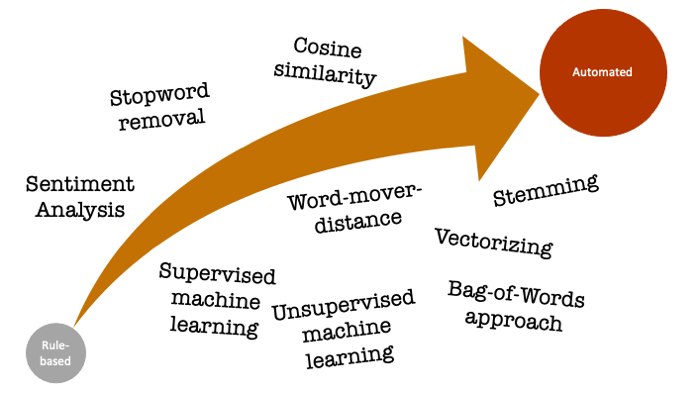
\includegraphics[width=\linewidth,height=\textheight,keepaspectratio]{Roadmap_terms.png}
	\end{center}
\end{frame}

\begin{frame}{Course structure}
\small

\textbf{Lectures}
\begin{itemize}
	\item Concepts, methods, examples, and implications
\end{itemize}

\vspace{-0.15cm}
\textbf{Tutorials}
\begin{itemize}
	\item Coding exercises
	\item Practice with course concepts
	\item Support for the group assignment
\end{itemize}

\vspace{-0.15cm}
\textbf{Assessment}
\begin{itemize}
	\item Multiple-choice questions (\(20\%\))
	\item Group assignment: written report (\(20\%\))
	\item Group assignment: presentation (\(15\%\))
	\item Exam (\(45\%\))
\end{itemize}
\end{frame}

\begin{frame}{Assessment details}
\begin{itemize}
	\item \textbf{Multiple-choice questions}
	\begin{itemize}
		\item 4 questions in weeks 1, 3, 4, 7, and 8
		\item 20 questions in total
		\item 16 correct answers = full marks
	\end{itemize}
	\item \textbf{Group assignment}
	\begin{itemize}
		\item Work in groups  
		\item Write a short report
		\item Build and present a recommender system
	\end{itemize}
	\item \textbf{Exam}
	\begin{itemize}
		\item Final tutorial session
		\item Conceptual questions + coding task
	\end{itemize}
\end{itemize}
\end{frame}

\begin{frame}{How to stay informed}
Regularly check:
\begin{itemize}
	\item The course Canvas page
	\item Your university email
	\item The course materials and announcements
\end{itemize}

\vspace{0.3cm}
Also: read the course manual carefully.
\end{frame}

\begin{frame}{A few practical notes}
\begin{itemize}
	\item Bring a laptop with a working Python environment
	\item Attend lectures and tutorials regularly
	\item Ask coding questions during tutorials
	\item Use AI tools responsibly and transparently
\end{itemize}
\end{frame}

\begin{frame}{Ready? Set? Go!}
	\begin{center}
		\Large Enough logistics\ldots \\[0.5cm]
		\Large \ldots let's get started.
	\end{center}
\end{frame}

\section{Text as data}

\begin{frame}{Why Computational Communication Science?}
\begin{columns}
\column{0.6\textwidth}

Digital communication produces large amounts of data:
\begin{itemize}
	\item news articles
	\item social media posts
	\item online reviews
	\item forum discussions
	\item archives and documents
\end{itemize}

Computational methods help us study this data systematically and at scale.

\column{0.4\textwidth}

\includegraphics[width=\linewidth]{doge-big-data-meme.jpg}
\end{columns}
\end{frame}

\begin{frame}{A simple roadmap for this course}
\small
Most of what we do in this course follows the same logic:

\begin{center}
\large
Text $\rightarrow$ Data $\rightarrow$ Representation $\rightarrow$ Model $\rightarrow$ Insight
\end{center}

\vspace{0.3cm}
Today we focus mainly on how text becomes usable data.
\end{frame}

\begin{frame}{Why do the basics still matter?}
Modern AI tools can automate many language tasks.

\begin{itemize}
    \item But the core questions remain the same:
    \begin{itemize}
        \item How is text represented?
        \item What patterns are being learned?
        \item How accurate are the outputs?
        \item What biases or errors may appear?
    \end{itemize}
\end{itemize}

\vspace{0.3cm}
\textbf{Takeaway:} Understanding basic text analysis helps you evaluate modern AI tools more critically.
\end{frame}

\begin{frame}{How computers analyze text}
\begin{center}
\large
Raw text

\vspace{0.1cm}
$\downarrow$

\vspace{0.1cm}
Preprocessing

{\small(tokenization, cleaning, stopword removal)}

\vspace{0.1cm}
$\downarrow$

\vspace{0.1cm}
Text representation

{\small(word counts, TF-IDF, embeddings)}

\vspace{0.1cm}
$\downarrow$

\vspace{0.1cm}
Models

{\small(classification, clustering, recommenders)}

\vspace{0.1cm}
$\downarrow$

\vspace{0.1cm}
Insights

{\small(patterns in communication data)}
\end{center}
\end{frame}

\begin{frame}{Text as data}
From CCS-1, you already know some basics:
\begin{itemize}
	\item how to work with Python
	\item how to store and read data
	\item how to work with strings, lists, and dictionaries
	\item how to loop through data and transform it
\end{itemize}

\vspace{0.3cm}
In CCS-2, we build on that foundation.
\end{frame}

\begin{frame}{Why study text?}
Text can be useful in at least two ways:
\begin{itemize}
    \item as the \textbf{object of study} itself
    \item as a \textbf{source of evidence} for a broader question
\end{itemize}
\end{frame}

\begin{frame}{Text as data: analyzing text as a goal}
Studying text can teach us a lot about communication:
\begin{itemize}
    \item We can study what people talk about on health platforms (e.g., \cite{sanders_different_2020})
    \begin{itemize}
        \item For example: which topics appear on expert-generated versus peer-generated platforms?
    \end{itemize}
    \item We can compare language across media environments (e.g., \cite{burggraaff_through_2020})
    \begin{itemize}
        \item For example: how does online news differ from print news?
    \end{itemize}
\end{itemize}
\end{frame}

\begin{frame}{Text as data: analyzing text as a means}
Text can also help answer broader research questions:
\begin{itemize}
\item We can use movie descriptions or reviews to study representation in media (e.g., \cite{poma-murialdo_gender_2019})
\item We can use webpage text to distinguish between reliable and unreliable information (e.g., \cite{meppelink_reliable_2021})
\item We can use content descriptions to build recommendation systems
\end{itemize}
\end{frame}

\begin{frame}{Computational Communication Science}
\begin{columns}[T]
	\begin{column}{0.6\textwidth}
		\begin{block}{What does the field do?}
			It uses computational methods to study communication and media data.
		\end{block}

		\vspace{0.2cm}
		\begin{itemize}
			\item \textbf{Data:} news, social media, forums, archives
			\item \textbf{Methods:} text analysis, machine learning, network analysis
			\item \textbf{Goal:} generate insight from digital communication
		\end{itemize}
	\end{column}

	\begin{column}{0.4\textwidth}
		
\includegraphics[width=\linewidth]{doge-big-data-meme.jpg}
	\end{column}
\end{columns}

\vspace{0.3cm}
\begin{block}{Why it matters}
It helps us study communication in natural, large-scale, digital settings.
\end{block}
\end{frame}

\begin{frame}{Challenges in computational research}

\begin{block}{Key challenges}
\begin{itemize}
	\item \textbf{Data access:} what data can we actually obtain?
	\item \textbf{Data validity:} are these data representative?
	\item \textbf{Measurement:} how accurate are automated measures?
	\item \textbf{Ethics:} how do we use data responsibly?
\end{itemize}
\end{block}

\vspace{0.4cm}
\begin{block}{Takeaway}
Computational methods are powerful, but they should always be used critically.
\end{block}

\vspace{0.2cm}
\small \textbf{Reference:} \cite{vanAtteveldt2018}
\end{frame}

\begin{frame}{Natural Language Processing (NLP)}
\begin{columns}[T]
	\begin{column}{0.65\textwidth}
		\begin{block}{Definition}
	Natural Language Processing (NLP) studies how computers can process and analyze human language.
		\end{block}

		\vspace{0.2cm}
		It often combines:
		\begin{itemize}
			\item language data
			\item computational rules
			\item machine learning
		\end{itemize}
	\end{column}

	\begin{column}{0.25\textwidth}
		\vspace{0.5cm}
		
\includegraphics[width=0.9\linewidth]{../pictures/sprinkle-it-in.jpg}
	\end{column}
\end{columns}
\end{frame}

\begin{frame}{Want to know more?}
Explore how large-scale text analysis changed research and public knowledge:

\vspace{0.4cm}
\begin{center}
\url{https://www.ted.com/talks/jean_baptiste_michel_erez_lieberman_aiden_what_we_learned_from_5_million_books}
\end{center}
\end{frame}

\section{Two approaches to text analysis}

\begin{frame}{Two ways to study text}
Imagine you study news about climate change.

\vspace{0.3cm}

You could:
\begin{itemize}
	\item explore the data to see which words and themes appear
	\item or measure the presence of predefined categories such as \emph{policy}, \emph{economy}, or \emph{crisis}
\end{itemize}

\vspace{0.4cm}
These correspond to two broad approaches.
\end{frame}

\begin{frame}[standout]
Automated content analysis often follows two main approaches:

\begin{itemize}
	\item \textcolor{red}{Bottom-up}: exploratory, pattern-based, data-driven
	\item \textcolor{red}{Top-down}: guided by predefined categories or rules
\end{itemize}

Sometimes researchers also combine both.
\end{frame}

\begin{frame}{The CCS toolbox in practice}
\centering
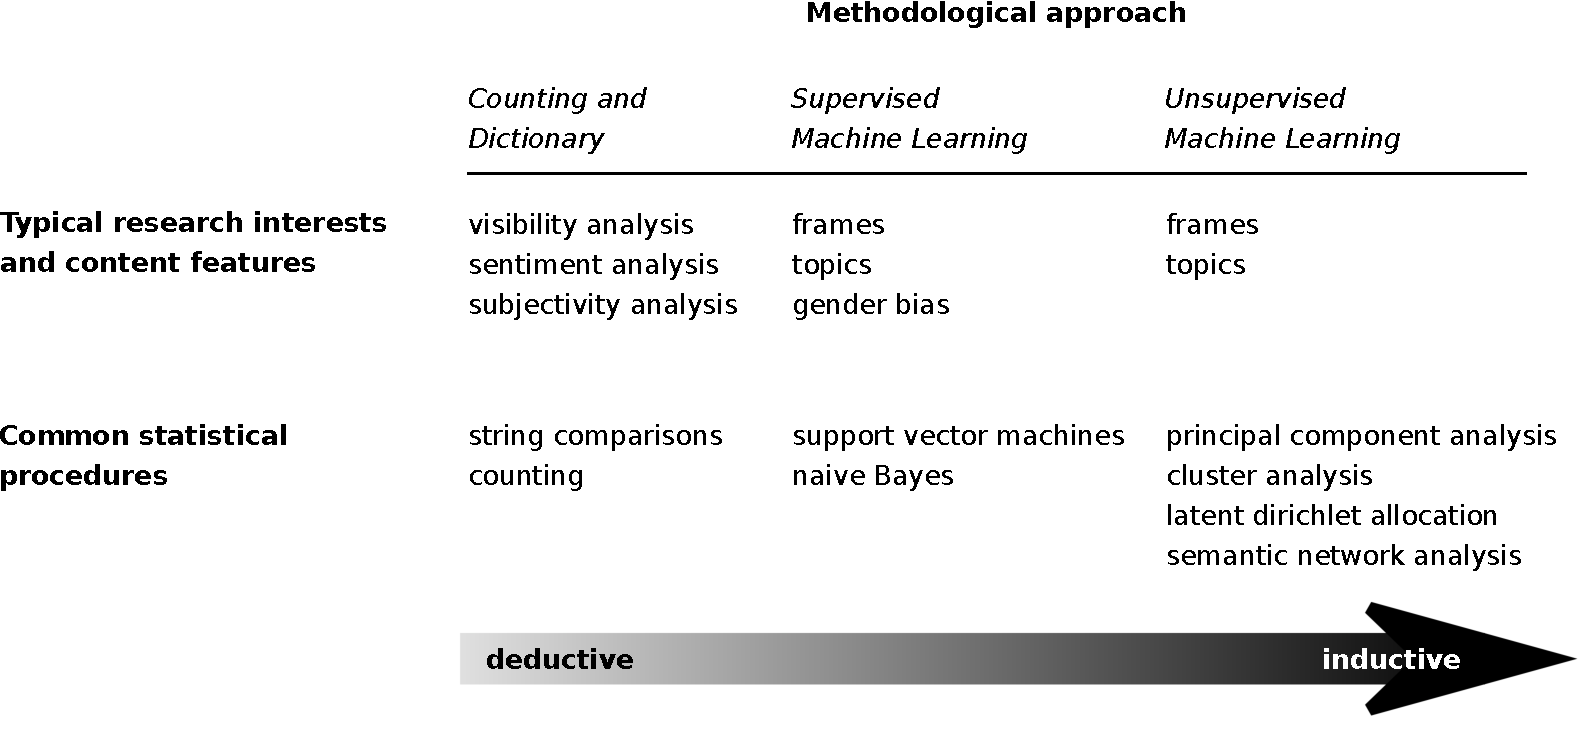
\includegraphics[width=0.9\columnwidth]{boumanstrilling2016}

\vspace{0.5cm}
\small{Source: \cite{Boumans2016}}
\end{frame}

\begin{frame}{Two approaches to automated content analysis}
\begin{columns}
\column{0.5\textwidth}
\begin{block}{\textbf{Bottom-up}}
\begin{itemize}
	\item discover patterns in data
	\item no fixed categories in advance
	\item useful for exploration
\end{itemize}
\end{block}

\column{0.5\textwidth}
\begin{block}{\textbf{Top-down}}
\begin{itemize}
	\item use predefined categories
	\item measure something specific
	\item useful for theory-driven analysis
\end{itemize}
\end{block}
\end{columns}
\end{frame}

\begin{frame}{Understanding the difference}
\begin{columns}
\column{0.5\textwidth}
\begin{block}{\textbf{Bottom-up}}
\begin{itemize}
	\item identify frequent words
	\item explore co-occurrence patterns
	\item ask: \emph{What seems to be going on here?}
\end{itemize}
\textbf{Key idea:} we do \emph{not} fully decide in advance what to look for.
\end{block}

\column{0.5\textwidth}
\begin{block}{\textbf{Top-down}}
\begin{itemize}
	\item count predefined terms
	\item detect known categories
	\item ask: \emph{How much of X do we see?}
\end{itemize}
\textbf{Key idea:} we \emph{do} decide in advance what to look for.
\end{block}
\end{columns}
\end{frame}

\begin{frame}{Research example of a bottom-up approach}
\begin{block}{Exploring prominent terms in disease-related texts}
\begin{itemize}
    \item identifies frequent words and patterns in text
    \item can reveal themes without predefined categories
    \item useful for exploratory research
\end{itemize}
\begin{center}
    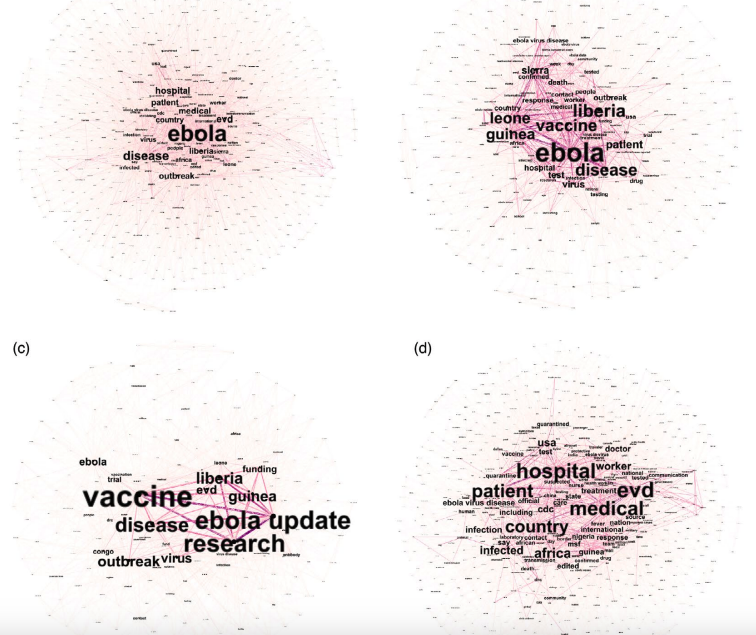
\includegraphics[width=0.4\linewidth]{wordcloud.png}\\
    \small \cite{you2021using}
\end{center}
\end{block}
\end{frame}

\begin{frame}{Research example of a top-down approach}
\begin{block}{Sentiment analysis using LIWC}
\begin{itemize}
	\item LIWC uses predefined word categories
	\item it counts words related to emotions, cognition, and social processes
	\item useful when researchers want structured, theory-driven measurement
\end{itemize}
\end{block}
\vspace{0.4cm}
\small \cite{tausczik2010psychological}
\end{frame}

\begin{frame}{LIWC application in online support groups}
\begin{itemize}
	\item LIWC was used to analyze language in online support groups for breast cancer patients \cite{shim2011does}
	\item It categorizes words into emotional and cognitive dimensions
	\item This helped researchers connect language use to well-being outcomes
\end{itemize}

\begin{center}
	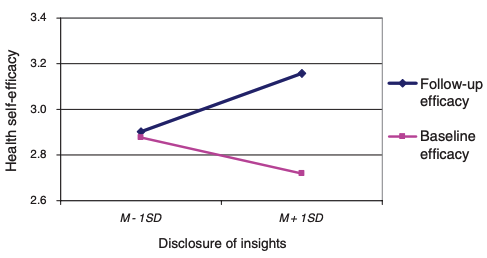
\includegraphics[width=0.75\linewidth]{../pictures/LIWC.png}
\end{center}
\end{frame}

\begin{frame}{Why both approaches matter}
\begin{itemize}
	\item \textbf{Bottom-up} is useful when you want to explore
	\item \textbf{Top-down} is useful when you want to measure something specific
	\item In practice, researchers often combine both
\end{itemize}

\vspace{0.3cm}
\textbf{Example:} first explore which themes appear, then build a more focused measurement.
\end{frame}

\subsection{Hands-on examples}

\begin{frame}[fragile]{A simple bottom-up approach}
\textbf{Goal:} Identify frequent words in a small text collection.

\begin{minted}{python}
from collections import Counter

texts = ["Communication in the digital society is very very complex", 
		 "I like to study it"]

bottom_up = []
for text in texts:
    counts = Counter(text.lower().split())
    bottom_up.append(counts.most_common(3))

print(bottom_up)
\end{minted}

\pause

This produces:

\begin{minted}{text}
[[('very', 2), ('communication', 1), ('in', 1)],
 [('i', 1), ('like', 1), ('to', 1)]]
\end{minted}
\textbf{Note:} This is a toy example that counts words within each text separately.
\end{frame}

\begin{frame}[fragile]{A simple top-down approach}
\textbf{Goal:} Count specific words that we care about in advance.

\begin{minted}{python}
texts = ["Communication in the digital society is very very complex", 
		 "I like to study it"]

features = ["communication", "digital", "study"]

top_down = []
for text in texts:
    words = text.lower().split()
    counts = [words.count(feature) for feature in features]
    top_down.append(counts)

print(top_down)
\end{minted}

\pause

This produces:

\begin{minted}{text}
[[1, 1, 0], [0, 0, 1]]
\end{minted}
\end{frame}

\question{When would you use which approach?}

\begin{frame}{Some considerations}
\begin{itemize}
	\item Both approaches can be useful
	\item Bottom-up is often a good exploratory first step
	\item Top-down is often useful when you have a clear concept or theory
	\item In both cases, text must be turned into something that can be counted or compared
\end{itemize}
\end{frame}

\section{Preprocessing}

\begin{frame}{Preprocessing text}
\begin{block}{Why preprocess?}
Before we can analyze text, we usually need to transform it into a more structured format.
\end{block}

\begin{itemize}
	\item This is often the first step in NLP
	\item It prepares text for later analysis
	\item We will revisit these ideas throughout the course
\end{itemize}
\end{frame}

\begin{frame}{Preprocessing: what matters today}
For now, focus on two basic questions:
\begin{itemize}
	\item How do we split text into smaller units?
	\item How do we clean text so it becomes easier to analyze?
\end{itemize}

\vspace{0.3cm}
Later in the course, we will return to more advanced preprocessing choices.
\end{frame}

\begin{frame}{Typical preprocessing steps}
\begin{block}{A basic preprocessing pipeline}
\begin{description}
    \item[\emph{Tokenization}] splitting text into tokens
    \item[\emph{Cleaning / filtering}] removing or normalizing unwanted elements
    \item[\emph{Stopword removal}] removing very frequent words when appropriate
    \item[\emph{Lemmatization / stemming}] reducing variation in word forms
\end{description}
\end{block}

\vspace{0.3cm}
Today we mainly focus on tokenization and simple cleaning.
\end{frame}

\begin{frame}[fragile]{Simple string methods}
\begin{block}{Slicing}
\texttt{mystring[2:5]} gets the characters with indices 2, 3, and 4
\end{block}

\begin{block}{Useful string methods}
\begin{itemize}
	\item \texttt{.lower()} returns a lowercased string
	\item \texttt{.strip()} removes whitespace at the beginning and end
	\item \texttt{.find("bla")} returns the index of a substring or -1
	\item \texttt{.replace("a","b")} replaces one string with another
	\item \texttt{.count("bla")} counts how often a substring occurs
\end{itemize}
Use tab completion to discover more.
\end{block}
\end{frame}

\begin{frame}[fragile]{A first simple tokenizer: \texttt{.split()}}
\begin{block}{Idea}
\texttt{.split()} cuts text where there are spaces.
\end{block}

\begin{itemize}
	\item easy to use
	\item useful for learning
	\item limited when punctuation and contractions matter
\end{itemize}

\begin{minted}{python}
docs = ["This is a text", "I haven't seen John's derring-do. Second sentence!"]
tokens = [doc.split() for doc in docs]
tokens
\end{minted}

\begin{minted}{text}
[['This', 'is', 'a', 'text'],
 ['I', "haven't", 'seen', "John's", 'derring-do.', 'Second', 'sentence!']]
\end{minted}
\end{frame}

\begin{frame}[fragile]{A slightly better tokenizer}
\begin{block}{Tokenizers from NLTK}
Packages such as NLTK provide tokenizers that handle text more carefully.
\end{block}

\begin{itemize}
	\item better with punctuation
	\item better with contractions
\end{itemize}

\begin{minted}{python}
from nltk.tokenize import TreebankWordTokenizer

tokenizer = TreebankWordTokenizer()
tokens = [tokenizer.tokenize(doc) for doc in docs]
tokens
\end{minted}

\pause

\begin{minted}{python}
[['This', 'is', 'a', 'text'],
 ['I', 'have', "n't", 'seen', 'John', "'s", 'derring-do.', 'Second', 'sentence', '!']]
\end{minted}

\pause
\small \textbf{Note:} Better does not mean perfect — tokenizers still make rule-based choices.
\end{frame}

\begin{frame}[fragile]{Tokenizing and removing punctuation}
\begin{minted}{python}
from nltk.tokenize import RegexpTokenizer

tokenizer = RegexpTokenizer(r'\w+')

text = "Hi students, what's up!"
tokens = tokenizer.tokenize(text)

print(tokens)
\end{minted}

\pause

\begin{minted}{python}
['Hi', 'students', 'what', 's', 'up']
\end{minted}

\pause

\textbf{Regex:} \texttt{\textbackslash w+} = one or more word characters

\pause

\textbf{Note:}
\begin{itemize}
\item Removes punctuation
\item Splits contractions ("what's" → "what", "s")
\end{itemize}
\end{frame}

\begin{frame}{Choosing a tokenizer}

\textbf{There is no perfect tokenizer — it depends on your goal}

\vspace{1em}

\begin{itemize}
\item \texttt{split()}  
→ very simple (spaces only)  
→ good for first introduction  

\vspace{0.5em}

\item \texttt{TreebankWordTokenizer}  
→ handles punctuation and contractions  
→ good for linguistic analysis  

\vspace{0.5em}

\item \texttt{RegexpTokenizer}  
→ removes punctuation, keeps words  
→ good for counting and simple models  
\end{itemize}

\end{frame}

\begin{frame}{Stopwords}
\begin{block}{What are stopwords?}
\begin{itemize}
	\item very frequent words with limited analytical value
	\item examples: \texttt{the, a, is, he, she}
	\item what counts as a stopword depends on your research question
\end{itemize}
\end{block}

\vspace{0.3cm}
For example, if you study gender, \texttt{he} and \texttt{she} may be very important.
\end{frame}

\begin{frame}{Why remove stopwords?}
\begin{itemize}
	\item to highlight more meaningful words
	\item to reduce noise in comparisons between documents
	\item to improve some visualizations and simple analyses
\end{itemize}

\vspace{0.3cm}
But: removing stopwords is not always the right choice.
\end{frame}

\begin{frame}[fragile]{Stopword removal}
\begin{minted}{python}
from nltk.corpus import stopwords

mystopwords = stopwords.words("english")
mystopwords.extend(["this", "is"])

tokens_without_stopwords = [
    [word.lower() for word in doc if word.lower() not in mystopwords]
    for doc in tokens
]

tokens_without_stopwords
\end{minted}

\begin{minted}{python}
[['text'], ["n't", 'seen', 'John', 'derring-do.', 'Second', 'sentence', '!']]
\end{minted}
\end{frame}


\begin{frame}{A note on modern NLP tools}
Many ideas we discuss today also appear in newer tools and workflows.

\begin{itemize}
\item \texttt{NLTK} is great for learning the basics
\item Other common tools include \texttt{spaCy} and transformer-based models
\item Even with newer tools, the core workflow is still:
	\begin{itemize}
		\item tokenize
		\item represent
		\item model
		\item evaluate
	\end{itemize}
\end{itemize}
\end{frame}

\begin{frame}{Do we still need preprocessing?}

\textbf{Short answer: yes --- but it depends on your method}

\vspace{0.7em}

\textbf{When preprocessing is important:}
\begin{itemize}
\item Counting words (e.g., frequency, TF-IDF)
\item Dictionary-based analysis (e.g., sentiment, LIWC)
\item Simple models or recommender systems
\end{itemize}

\end{frame}

\begin{frame}{Do we still need preprocessing?}

\textbf{When less preprocessing is needed:}
\begin{itemize}
\item Modern AI models (e.g., BERT, GPT)
\item Handle tokenization and variation internally
\end{itemize}

\vspace{0.7em}

\textbf{Key idea:}
\begin{itemize}
\item If \textbf{you design features} → preprocessing matters
\item If \textbf{model learns features} → less preprocessing
\end{itemize}

\end{frame}


\begin{frame}{Tomorrow's tutorial}
\begin{block}{Tutorial meeting}
\begin{itemize}
	\item Discuss course goals and policies
	\item Revisit some CCS-1 basics
	\item Practice simple top-down and bottom-up text analysis
	\item Start thinking about the group assignment
	\end{itemize}
\end{block}
\end{frame}

\begin{frame}{Key takeaways}
\begin{itemize}
	\item Digital communication produces large amounts of textual data
	\item Computational methods help us analyze text systematically
	\item For most computational analysis, text must be represented in a structured form.
	\item Bottom-up and top-down approaches each have strengths
	\item Preprocessing is an important first step 
\end{itemize}
\end{frame}

\begin{frame}{Practice is key!}
    \centering
    
\includegraphics[width=0.8\textwidth,height=0.8\textheight,keepaspectratio]{python_running.jpeg}
\end{frame}

\begin{frame}{Thank you!}
\begin{block}{Thank you for your attention}
\begin{itemize}
	\item Questions?
	\item Comments?
\end{itemize}
\end{block}
\end{frame}

\begin{frame}[t,allowframebreaks]
	\frametitle{References}
	\printbibliography
\end{frame}

\end{document}